\chapter{MICROSTRUCTURE ANALYSIS IN METALLIC MATERIALS}
\section{Experimental targets}
\begin{itemize}
	\item To Learn the preparation of specimen for microscopic observation.
	\item To understand what microscopy is, and how it can be used to observe Microstructure of metals.
\end{itemize}
\section{Theoretical summary}
\begin{itemize}
	\item \textbf{Metallography:} Is the study of metals by optical and electron microscopes.
	\item \textbf{Optical microscopy}: With  optical  microscopy,  the  light  microscope  is  used  to  study  the microstructure; optical illumination systems are its basic elements.
	\item \textbf{Sectioning:} Operations  such  as  shearing  produce  severe  cold  work,  which  can  alter  the microstructure of a sample.
	\item \textbf{Mounting:} Small samples are generally mounted in plastic for convenience in handling and to protect the edges of the specimen being prepared.
	\item \textbf{Coarse Grinding}: The purpose of the coarse grinding stage is to generate the initially flat surface necessary for the subsequent grinding and polishing steps. Course grinding can be accomplished either wet or dry using 80 to 180 grit electrically powered disks or belts, but care must be taken to avoid significant heating of the sample.
	\item \textbf{Medium and Fine Grinding:} To produce a scratch free surface by employing a series of successively finer abrasives.
	\item \textbf{Mechanical Polishing:} Polishing involves the use of abrasives, suspended in a water solution, on a cloth-covered electrically powered wheel.
	\item \textbf{Etching:} Microscopic examination of a properly polished, unetched specimen will reveal only a few structural features such as inclusions and cracks or other physical imperfections. Etching is used to highlight, and sometimes identify, microstructural features or phases present.
\end{itemize}
\section{Detailed experiment}
\begin{itemize}
	\item Cut out the work piece.
	\item Coarse grinding: Use sand paper from small to big number (80,100,150,180,400).
	\item Polishing: Use polishing machine attached by cloth soaked in water.
	\item Get the surface image from the microscope.
	\item Etching: Use acid to remove the outer layer of the surface, then clean the surface with water.
	\item Get the surface image again from the microscope.
\end{itemize}

\section{Microstructure before and after etching}
\begin{figure}[ht]
	\centering
	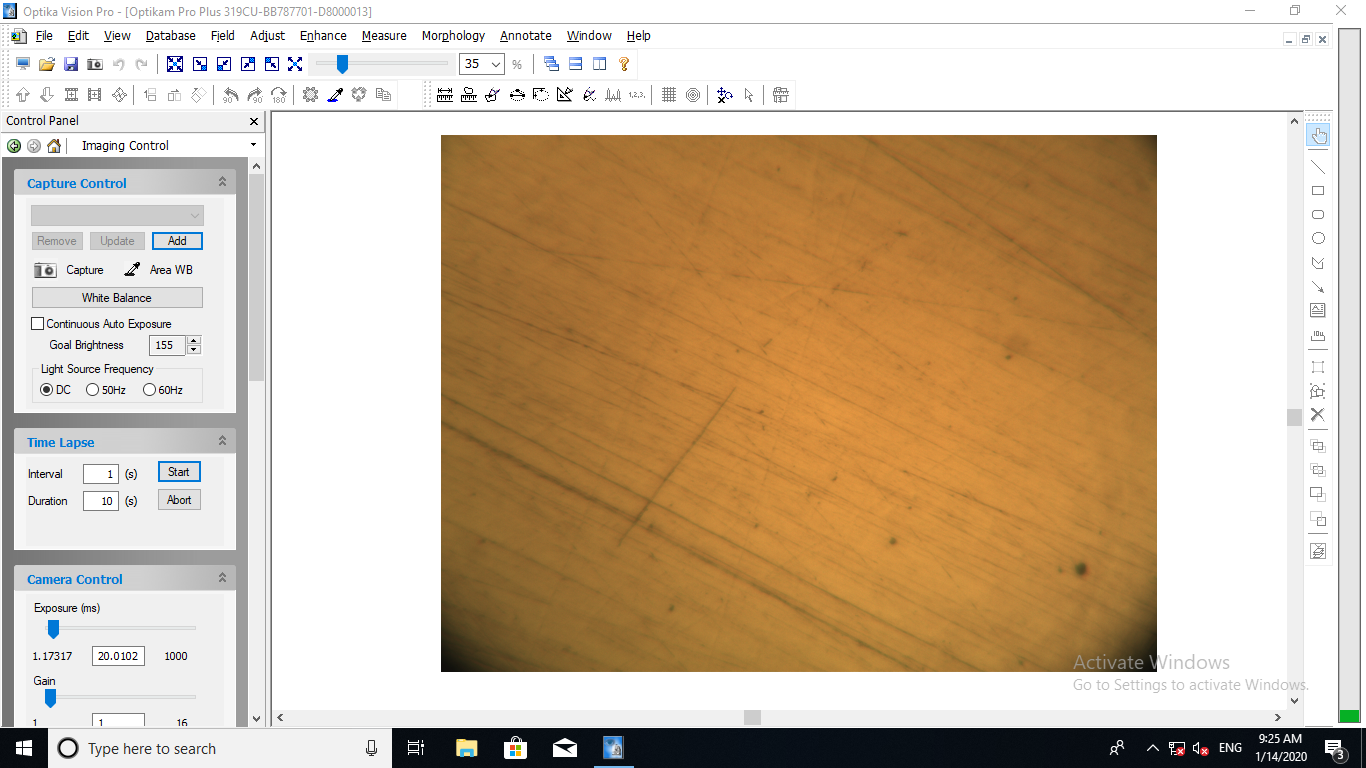
\includegraphics[width=150mm]{1852158-1852269.png}
	\caption{Microstructure of the sample before etching}
\end{figure}
\begin{figure}[ht]
	\centering
	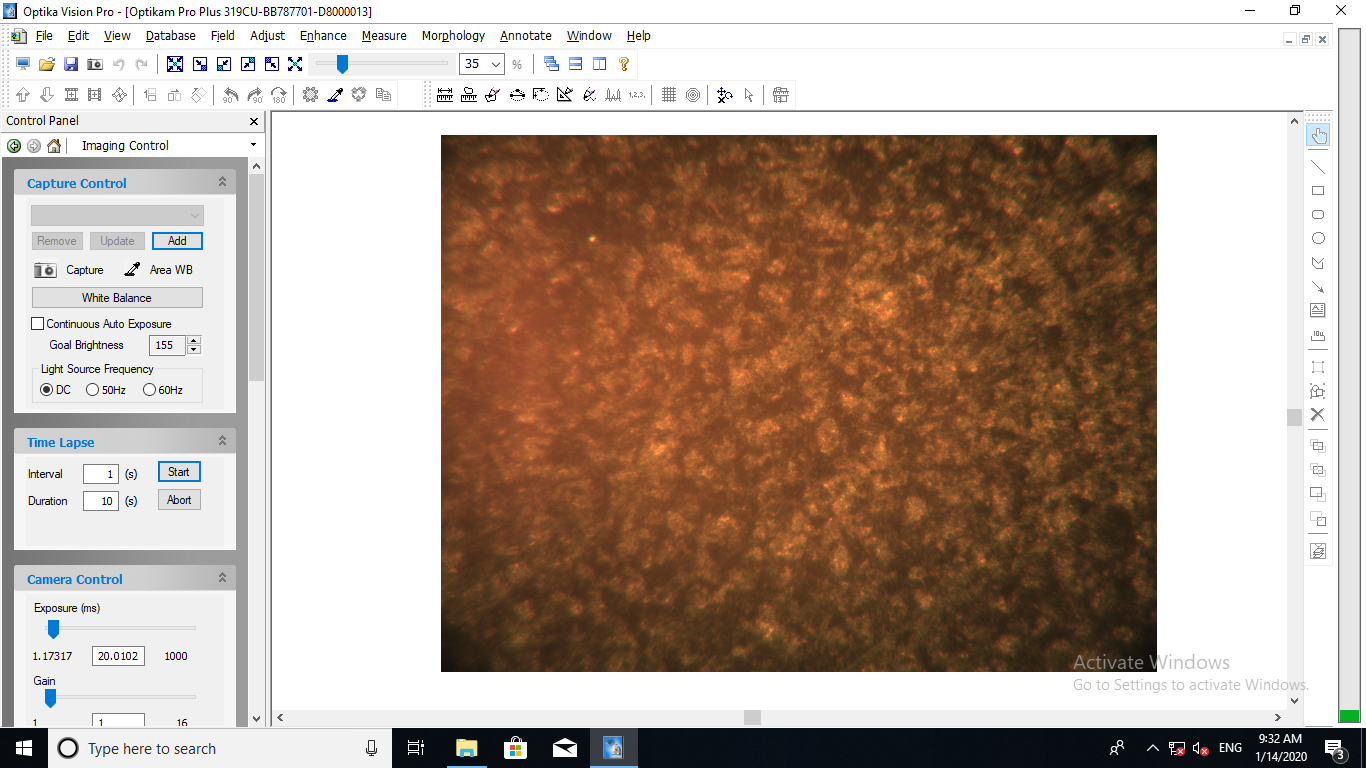
\includegraphics[width=150mm]{1852158-1852269-2.png}
	\caption{Microstructure of the sample after etching}
\end{figure}

\section{Conclusion}
Before food etching:
\begin{itemize}
	\item The pre-impregnated sample is very bright with the naked eye due to careful polishing. However, the scratches are still visible and crossing each other under the microscope.
	\item In conclusion, the process of sanding and polishing are guaranteed to reduce the scratches. However, abusing this process too much will peel off the hardened surface of the sample, which makes it prone to environmental damages. 
\end{itemize}
 
After food etching:
\begin{itemize}
	\item After impregnation, the surface becomes blur because of porous at microscopic scale, which is evident by black spots on the images above. If the sample is exposed to air, the surface will become darker.
	\item The reaction of the sample surface with the etching solution is not the same at all points.
	\item The more polished the sample is, the easier it is to see the results after impregnating it, then it is easy to see the border between particles and phases together through a microscope.
	\item The more impregnated at the required time, the more visible the results will be because the grain and phase boundaries have not been corroded too much. 
\end{itemize}

In summary:
\begin{itemize}
	\item The given sample has different phases lying alternately so that the reactions are not homogeneous on the sample surface.
	\item When etching the phases on the sample, it is unevenly corroded or there are some phases that are corroded faster, the irregular corrosion creates a rough surface for the sample (surface roughness).
	\item The given sample has soft and hard phases interspersed together to form a uniform mass.
	\item The boundaries between the phases and the particles are quite even, with no major defects. 
\end{itemize}
